\chapter{Generalidades}
<<<<<<< HEAD
	
	
	\section{Objetivos}\label{sec:2.1}

\subsection{Objetivo general}\label{sec:2.1.1}

Desarrollar un Sistema  Integral de Indicadores que permita medir, evaluar y controlar los procesos realizados por cada departamento en el Instituto Tecnol\'ogico de Tl\'ahuac, basado en los lineamientos establecidos por la TecNM en el Sistema de Gesti\'on de Calidad, para lograr realizar una gesti\'on eficaz y de calidad de los mismos.\\

Lorem ipsum dolor sit amet, consectetur adipiscing elit. Proin sagittis sem non ex dapibus, tincidunt malesuada tortor posuere. Suspendisse rutrum fermentum turpis, at feugiat est cursus ac. Praesent ac gravida enim. Fusce eget eleifend nisi. Nulla facilisi. Nam porta diam nec nulla aliquam, sed mollis augue scelerisque. Sed non tempus quam. Aliquam et sem fringilla, pretium leo et, semper justo. Quisque ultrices elementum mi, ac placerat purus suscipit nec. Nulla ligula sem, tristique in vehicula non, malesuada at quam. Phasellus posuere neque ac ultricies pharetra.

\subsection{Objetivos espec\'ificos}\label{sec:2.1.2}
\begin{itemize}
    \item Eficaz an\'alisis de requerimientos. 
    \item Correcta toma de datos y adecuadas entrevistas.
    \item Adecuado desarrollo del sistema.
    \item Implementaci\'on oportuna de pruebas de funcionamiento.
    \item Implemetaci\'on de pruebas en ambiente y de producci\'on.
\end{itemize}

\section{Justificaci\'on}\label{sec:2.2}
\paragraph{}%parrafo 1

Dicho proyecto basado en una herramienta que permitir\'a la evaluaci\'on autom\'atica de los procesos indicados en el Sistema de Gesti\'on de Calidad del Instituto Tecnol\'ogico de Tl\'ahuac, esto debido a que no se cuenta con ningun sistema para la realizaci\'on de dicha evaluaci�\'on, ya que actualmente los procesos se realizan de manera manual, teniedno as\'i procesos extensos y complicados\\

Facilitar\'a el trabajo realizado, agilizar\'a los tiempos requeridos y permitir\'a con esto brindar un mejor servicio a la comunidad del Instituto Tecnol\'ogico de Tl\'ahuacuna, contando as\'i con Indicadores para la toma de desiciones e influyendo en el cumplimiento de los objetivos. Logrando como beneficio el perfeccionamiento de la Intituci\�n\\

Lorem ipsum dolor sit amet, consectetur adipiscing elit. Proin sagittis sem non ex dapibus, tincidunt malesuada tortor posuere. Suspendisse rutrum fermentum turpis, at feugiat est cursus ac. Praesent ac gravida enim. Fusce eget eleifend nisi. Nulla facilisi. Nam porta diam nec nulla aliquam, sed mollis augue scelerisque. Sed non tempus quam. Aliquam et sem fringilla, pretium leo et, semper justo. Quisque ultrices elementum mi, ac placerat purus suscipit nec. Nulla ligula sem, tristique in vehicula non, malesuada at quam. Phasellus posuere neque ac ultricies pharetra.
\paragraph{}%parrafo 2
Lorem ipsum dolor sit amet, consectetur adipiscing elit. Proin sagittis sem non ex dapibus, tincidunt malesuada tortor posuere. Suspendisse rutrum fermentum turpis, at feugiat est cursus ac. Praesent ac gravida enim. Fusce eget eleifend nisi. Nulla facilisi. Nam porta diam nec nulla aliquam, sed mollis augue scelerisque. Sed non tempus quam. Aliquam et sem fringilla, pretium leo et, semper justo. Quisque ultrices elementum mi, ac placerat purus suscipit nec. Nulla ligula sem, tristique in vehicula non, malesuada at quam. Phasellus posuere neque ac ultricies pharetra.

\section{Caracterizaci\'on de la empresa en la que particip\'o}\label{sec:2.3}

\subsection{Datos generales de la empresa}\label{sec:2.3.1}
\begin{itemize}
         \item \textbf{Empresa:} 
         \item \textbf{Direcci�n:} 
         \vspace*{1in}
         \begin{figure}[htb]
            \centering
            %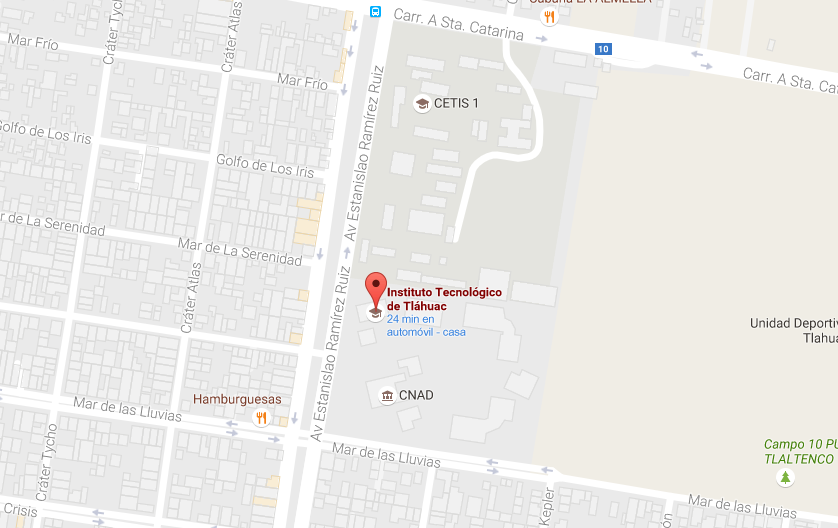
\includegraphics{croquis}
            \caption{Croquis de ubicaci�n.} \label{fig:croquis}
         \end{figure}
         \item \textbf{Tel�fono:} 
         \item \textbf{Direcci�n de correo electr�nico:} 
         \item Giro, misi�n, visi�n valores y pol�ticas de calidad:
         \item \textbf{Estructura organizacional:}
    \end{itemize}
=======
    
    
    \section{Objetivos}
>>>>>>> origin/UrbanoBallesteros

\subsection{Objetivo general}

<<<<<<< HEAD
\section{Problemas a resolver (prioriz\'andolos)}\label{sec:2.4}
\paragraph{}

Hasta hoy las evaluaciones de la calidad de los procesos se lleva a cabo de manera manual por cada uno de los Departamentos de dicha Instituci\'on, debido a que no se cuenta con una herramienta especilizada para realizarlo de manera rapida y eficaz, por lo que es necesario desarrollar un sistema para facilitar la evaluac\'on de dichos procesos\\


Lorem ipsum dolor sit amet, consectetur adipiscing elit. Proin sagittis sem non ex dapibus, tincidunt malesuada tortor posuere. Suspendisse rutrum fermentum turpis, at feugiat est cursus ac. Praesent ac gravida enim. Fusce eget eleifend nisi. Nulla facilisi. Nam porta diam nec nulla aliquam, sed mollis augue scelerisque. Sed non tempus quam. Aliquam et sem fringilla, pretium leo et, semper justo. Quisque ultrices elementum mi, ac placerat purus suscipit nec. Nulla ligula sem, tristique in vehicula non, malesuada at quam. Phasellus posuere neque ac ultricies pharetra.
\vspace*{0.6in}
=======
Desarrollar un Sistema  Integral de Indicadores que permita medir, evaluar y controlar los procesos realizados por cada departamento en el Instituto Tecnol\'ogico de Tlahuac, basado en los lineamientos establecidos por la TecNM en el Sistema de Gesti\'on de Calidad, para lograr realizar una gesti\'on eficaz y de calidad de los mismos.\\
>>>>>>> origin/UrbanoBallesteros

